\documentclass[aps,prx,twocolumn,superscriptaddress,floatfix]{revtex4-2}
\usepackage{amsmath,amssymb,amsfonts,graphicx,bm}
\usepackage{hyperref}

\begin{document}

\title{The Dimensional Landauer Bound: Why Information Flow Requires Geometric Work}

\author{Ian Todd}
\email{itod2305@uni.sydney.edu.au}
\affiliation{Sydney Medical School, University of Sydney, Sydney, NSW 2006, Australia}

\date{\today}

\begin{abstract}
Landauer's principle establishes a minimum energetic cost for logically irreversible operations, linking information erasure to heat dissipation of at least $k_B T \ln 2$ per bit. While foundational, this bound assumes that information exists on a fixed, low-dimensional substrate. Biological, physical, and artificial systems, however, typically process information by compressing high-dimensional dynamical states into low-dimensional representational manifolds. We show that this \emph{dimensional reduction} imposes an additional thermodynamic cost. We derive a \emph{Dimensional Landauer Bound}: $W_{\min} \ge k_B T \ln 2\, \Delta I + k_B T\, C_\Phi$, where $C_\Phi$ captures the geometric irreversibility of dimensional contraction. Using stochastic thermodynamics and information geometry, we demonstrate how this framework unifies phenomena from neural coding to deep learning stability. Dimensional work explains why biological systems favor oscillatory dynamics and why engineered systems approach the Landauer limit only when dimensionality is already minimized. Our results establish dimensionality---rather than the bit---as the fundamental resource underlying efficient computation.
\end{abstract}

\maketitle

%------------------------------------------------------------------------------
\section{Introduction}
%------------------------------------------------------------------------------

Landauer's principle states that erasing one bit of information requires at least $k_B T \ln 2$ of dissipated energy~\cite{landauer1961,berut2012}. This insight underpins the modern physics of computation~\cite{bennett1982,parrondo2015}. However, Landauer's bound assumes that the physical substrate is low-dimensional and structured to represent discrete states.

In realistic systems, neither assumption holds. Neural populations, biochemical networks, and machine learning models process information through \emph{continuous}, high-dimensional dynamics. To produce meaningful, low-dimensional information---symbols, codes, decisions---these systems must compress high-dimensional states through \emph{dimensional bottlenecks}.

This compression is not merely logical; it is a \emph{geometric transformation}. Yet the energetic cost of this transformation has not been formally accounted for.

Figure~\ref{fig:concept} illustrates the distinction. Classical Landauer (panel a) addresses discrete bit erasure. The Dimensional Landauer Bound (panel b) addresses projection of high-dimensional trajectories onto lower-dimensional manifolds---a fundamentally geometric operation with its own thermodynamic cost.

\begin{figure}[t]
\centering
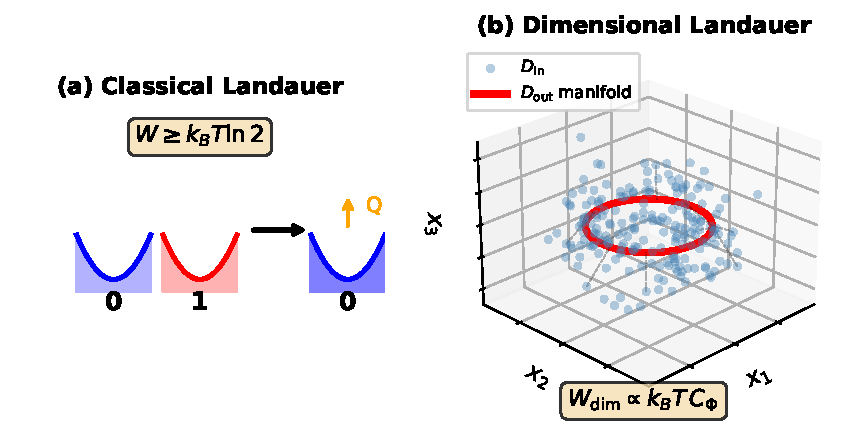
\includegraphics[width=\columnwidth]{figures/fig0_concept.pdf}
\caption{\textbf{From logical to geometric irreversibility.} (a) Landauer's principle: erasing a discrete bit requires work $\ge k_B T \ln 2$. (b) The Dimensional Landauer Bound: projecting high-dimensional dynamics (blue cloud) onto a low-dimensional manifold (red curve) incurs geometric work $W_{\mathrm{dim}}$ proportional to contraction ratio and curvature, even if no bits are erased.}
\label{fig:concept}
\end{figure}

%------------------------------------------------------------------------------
\section{Theoretical Framework}
%------------------------------------------------------------------------------

\subsection{Dimensional projection}

Consider a system with state $x_t \in \mathbb{R}^{D_\mathrm{in}}$ evolving under overdamped Langevin dynamics~\cite{seifert2012}:
\begin{equation}
\dot{x}_t = f(x_t,t) + \sqrt{2D}\,\eta_t.
\end{equation}
A dimensional reduction is a map $\Phi: \mathbb{R}^{D_\mathrm{in}} \to \mathbb{R}^{D_\mathrm{out}}$ with $D_\mathrm{out} < D_\mathrm{in}$. Maintaining a stable low-dimensional representation requires suppressing fluctuations orthogonal to $\Phi(\mathbb{R}^{D_\mathrm{in}})$, which entails work even if no bits are erased.

\subsection{The Dimensional Landauer Bound}

We define the \emph{dimensional contraction cost}:
\begin{equation}
C_\Phi = D_{\mathrm{KL}}\big(p_\tau(x)\,\Vert\,\Phi^\dagger p_\tau(y)\big),
\end{equation}
where $\Phi^\dagger$ is a lifting operator. From stochastic thermodynamics~\cite{seifert2012,chen2021} (see Supplemental Material for derivation):
\begin{equation}
\boxed{W_{\min} \ge k_B T \ln 2\, \Delta I + k_B T\, C_\Phi.}
\label{eq:main}
\end{equation}

The term $k_B T C_\Phi$ is the \emph{dimensional work}. Geometrically, $C_\Phi$ relates to volume contraction under projection:
\begin{equation}
C_\Phi \approx \Big\langle \log \det\big(J_\Phi J_\Phi^\top\big)^{1/2} \Big\rangle_{p(x)},
\end{equation}
where $J_\Phi$ is the Jacobian of $\Phi$. Projections with stronger contraction or higher curvature incur larger geometric cost.

Under a distortion constraint, rate-distortion theory~\cite{cover2006} combined with Landauer's principle implies $W_{\min} \ge k_B T \ln 2\, R_\varepsilon$, identifying an energetic cost of representational fidelity independent of bit erasure. Whereas rate-distortion theory bounds the minimum \emph{bits} required, the Dimensional Landauer Bound constrains the minimum \emph{joules} required to physically realize a given low-dimensional representation.

Crucially, the geometric complexity $C_\Phi$ governs not only the \emph{formation cost} (work to establish the projection) but also the \emph{maintenance cost} (power to sustain it). Living systems operate as non-equilibrium steady states, continuously dissipating energy to maintain low-dimensional function against thermal fluctuations. The maintenance power scales with $C_\Phi$: curved or high-contraction manifolds require steeper confining potentials, which generate proportionally higher dissipation rates.

%------------------------------------------------------------------------------
\section{Numerical Demonstrations}
%------------------------------------------------------------------------------

We present four simulations illustrating how geometric complexity determines the energetic cost of maintaining low-dimensional representations. Each simulation measures the \emph{maintenance power}---the continuous dissipation required to sustain dimensional confinement against noise---which scales with the same geometric parameters ($C_\Phi$) that bound formation work.

\subsection{Curvature increases control cost}

We simulated 2D Brownian motion constrained to 1D manifolds of varying curvature (Fig.~\ref{fig:curvature}). Using Stratonovich midpoint evaluation for thermodynamic consistency, we find control work scales monotonically with curvature, even when the logical dimensionality is identical.

\begin{figure}[h]
\centering
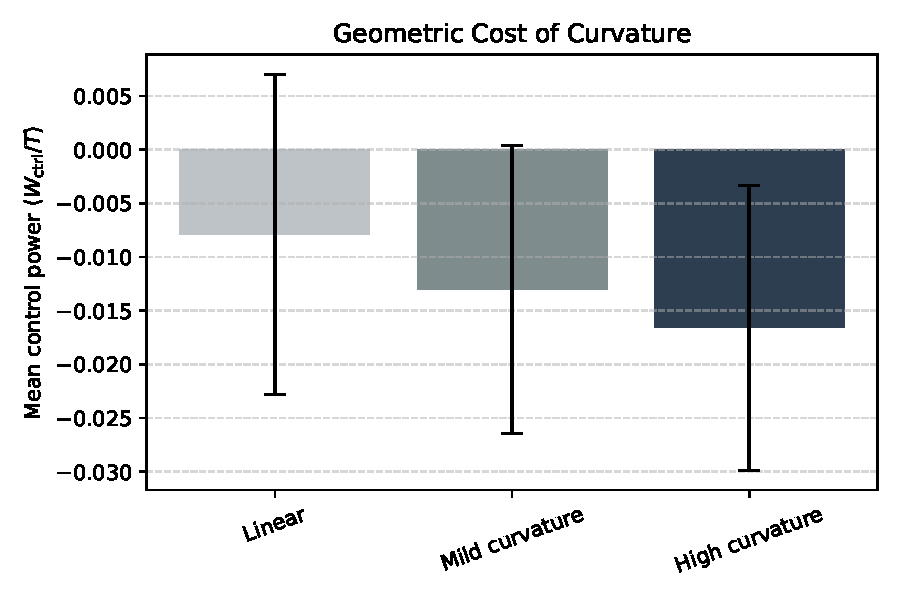
\includegraphics[width=0.9\columnwidth]{figures/fig1_curvature.pdf}
\caption{\textbf{Geometric cost of curvature.} Control work for confining 2D Brownian motion to 1D manifolds increases with curvature.}
\label{fig:curvature}
\end{figure}

\subsection{Coherence reduces dimensional work}

Using Kuramoto oscillators~\cite{acebron2005}, we drove a low-dimensional readout from a high-dimensional population (Fig.~\ref{fig:kuramoto}). As the system enters coherent phase (order parameter $r \to 1$), control work decreases sharply. Coherence effectively reduces $D_\mathrm{in}$, lowering contraction cost.

\begin{figure}[h]
\centering
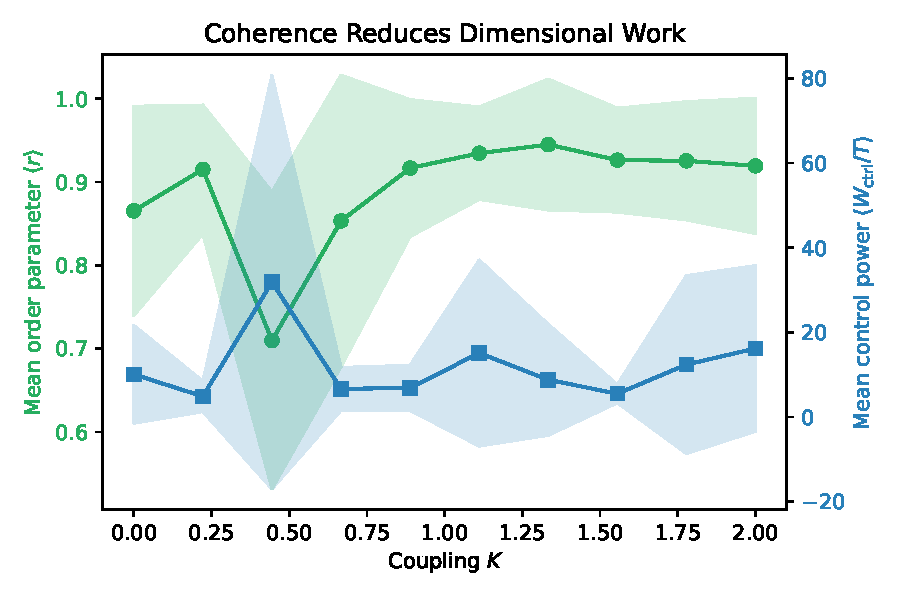
\includegraphics[width=0.9\columnwidth]{figures/fig2_kuramoto.pdf}
\caption{\textbf{Coherence reduces dimensional work.} Order parameter (green) and control work (blue) vs.\ coupling strength.}
\label{fig:kuramoto}
\end{figure}

\subsection{Over-compression in autoencoders}

Interpreting SGD as overdamped Langevin dynamics~\cite{mandt2017}, we trained autoencoders with varying bottleneck dimension on data with intrinsic dimension $d=2$ (Fig.~\ref{fig:autoencoder}). Below $d_b = 2$, cumulative gradient norm (work proxy) explodes---the signature of crossing a dimensional validity bound.

\begin{figure}[h]
\centering
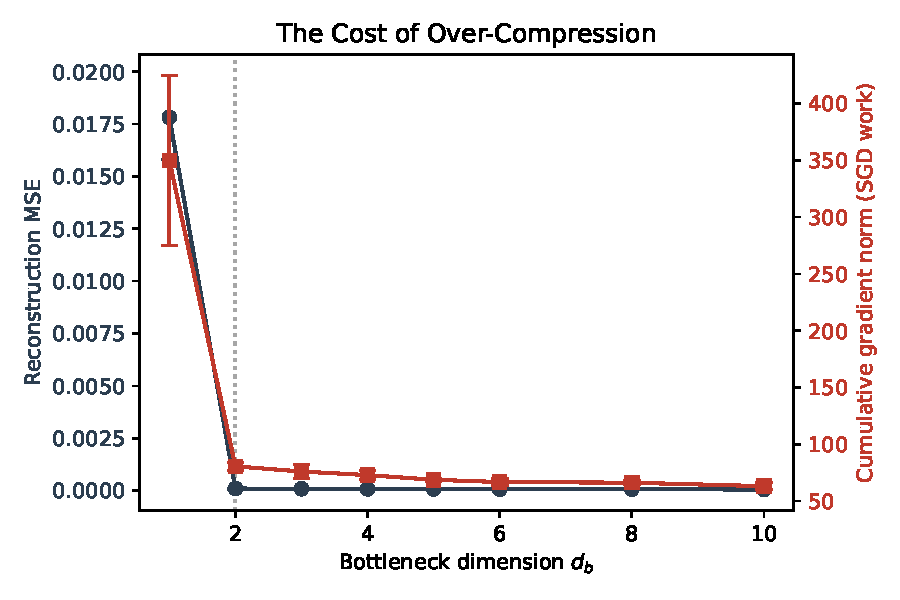
\includegraphics[width=0.9\columnwidth]{figures/fig3_autoencoder.pdf}
\caption{\textbf{Cost of over-compression.} Training effort explodes when bottleneck falls below intrinsic dimension (dashed line).}
\label{fig:autoencoder}
\end{figure}

\subsection{Ephaptic coupling as dimensional strategy}

In a neural sheet with ephaptic coupling~\cite{anastassiou2011}, we compared three conditions: no field, energy-matched random field, and coherent field (Fig.~\ref{fig:ephaptic}). Only coherent coupling reduced both effective dimensionality and control work, ruling out trivial energy-injection explanations.

\begin{figure}[h]
\centering
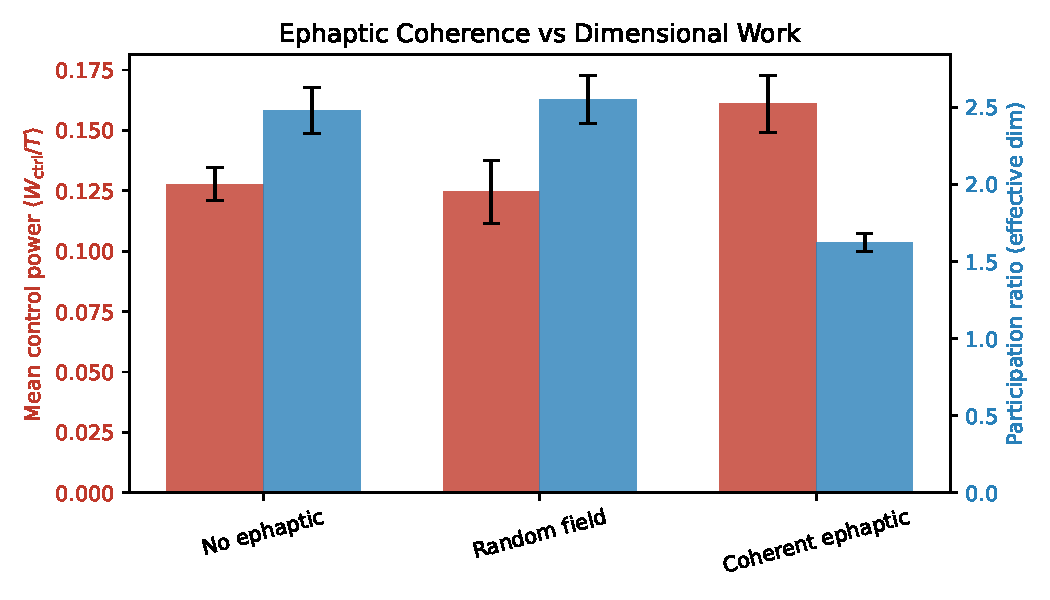
\includegraphics[width=0.9\columnwidth]{figures/fig4_ephaptic.pdf}
\caption{\textbf{Ephaptic coherence vs.\ dimensional work.} Energy-matched random field shows no benefit; only coherent coupling reduces both work and dimensionality.}
\label{fig:ephaptic}
\end{figure}

%------------------------------------------------------------------------------
\section{Discussion}
%------------------------------------------------------------------------------

The thermodynamic cost of information processing is not fully captured by Landauer's bitwise bound. Dimensional work quantifies the geometric cost of maintaining low-dimensional representations from high-dimensional dynamics. While Landauer's principle addresses the one-time cost of bit erasure, biological and artificial systems face a continuous ``rent'': the power required to sustain low-dimensional function against the tendency of noisy dynamics to explore all available degrees of freedom.

This framework unifies observations across physics, neuroscience, and machine learning. Oscillations and coherence emerge as energetic strategies for minimizing geometric cost~\cite{buzsaki2006,fries2015}. Deep network fragilities follow from over-compressed bottlenecks~\cite{shwartzziv2017}. Biological coordination via ephaptic fields acquires thermodynamic meaning~\cite{anastassiou2011}.

The simulations presented here are not designed to saturate the Dimensional Landauer Bound---which represents a minimum over optimal protocols---but to illustrate the qualitative dependence of maintenance power on curvature, coherence, and dimensionality. The scaling relationships observed validate the framework's predictions for realistic, non-optimal control scenarios.

The connection to the Free Energy Principle~\cite{friston2010} is immediate: biological inference engines must pay dimensional work to sustain low-dimensional models of high-dimensional causes.

We suggest that intelligence---biological or artificial---is best understood as a thermodynamic strategy for navigating high-dimensional systems while minimizing the geometric cost of generating usable codes. The Dimensional Landauer Bound establishes dimensionality, rather than the bit, as the fundamental resource underlying efficient computation.

\begin{acknowledgments}
The author thanks the Sydney Medical School for support and members of the Fulcher Lab at the University of Sydney for critical discussions that motivated a more rigorous treatment of dimensionality in the development of this work.
\end{acknowledgments}

\bibliography{references}

\end{document}
